\documentclass[12pt,a4paper]{article}
\usepackage[utf8]{inputenc}
\usepackage[T1]{fontenc}
%\usepackage[czech]{babel}
\usepackage{a4wide}
\usepackage{amsmath, amsthm, amsfonts, amssymb, graphicx, url, fancyhdr,multicol,enumerate,mathtools,tikz}
\newcommand{\norm}[1]{\left\lVert#1\right\rVert}

\newtheorem{theorem}{Theorem}
\newtheorem{lemma}[theorem]{Lemma}
\newtheorem{cor}[theorem]{Corollary}
\newtheorem{prop}[theorem]{Proposition}

\newcommand{\Cbb}{\mathbb{C}}
\newcommand{\Qbb}{\mathbb{Q}}
\newcommand{\Rbb}{\mathbb{R}}
\newcommand{\Zbb}{\mathbb{Z}}
\newcommand{\Nbb}{\mathbb{N}}
\newcommand{\C}{\mathbb{C}}
\newcommand{\Q}{\mathbb{Q}}
\newcommand{\R}{\mathbb{R}}
\newcommand{\Z}{\mathbb{Z}}
\newcommand{\F}{\mathbb{F}}
%\newcommand{\N}{\mathbb{N}}
\newcommand{\id}{\mathrm{id}}
\newcommand{\im}{\mathrm{im}}
\newcommand{\cok}{\mathrm{coker}}
\newcommand{\Hom}{\mathrm{Hom}}
\newcommand{\Max}{\mathrm{Max}}
\newcommand{\disc}{\mathrm{disc}}
\newcommand{\Gal}{\mathrm{Gal}}
\newcommand{\Tr}{\mathrm{Tr}}
\newcommand{\N}{\mathrm{N}}
\newcommand{\No}{\mathrm{N}_{\Qbb}^K}
\newcommand{\Ok}{\ensuremath{\mathcal{O}_K}}
\newcommand{\Ol}{\ensuremath{\mathcal{O}_L}}
\newcommand{\Cl}{\ensuremath{\mathcal{C}l}}
\newcommand{\p}{\mathfrak{p}}
\newcommand{\qq}{\mathfrak{q}}
\newcommand{\af}{\mathfrak{a}}
\newcommand{\bb}{\mathfrak{b}}
\newcommand{\rr}{\mathfrak{r}}
\newcommand{\al}{\alpha}
\newcommand{\z}{\zeta}
\newcommand{\zt}{\zeta_t}
\newcommand{\uo}{\overline{u}}
\newcommand{\vo}{\overline{v}}
\newcommand{\Mat}{\ensuremath{\text{Mat}(2,\mathbb{Z})}}
\newcommand{\Char}{\mathrm{char }}
\newcommand{\lcm}{\mathrm{lcm}}
\DeclarePairedDelimiter\abs{\lvert}{\rvert}

\newcommand\restr[2]{{% we make the whole thing an ordinary symbol
  \left.\kern-\nulldelimiterspace % automatically resize the bar with \right
  #1 % the function
  %\vphantom{\big|} % pretend it's a little taller at normal size
  \right|_{#2} % this is the delimiter
  }}

\begin{document}
%\pagestyle{fancy}                      %Pro větší­ možnosti práce se záhlaví­mi a zápatími
%\fancyhf{}                             %"vvyčištění záhlaví a zápatí"                                         
%\renewcommand{\headheight}{25 pt}                  %
\addtolength{\topmargin}{-30 pt}                   %
\setlength{\headsep}{10 pt}                      %
%\fancyhead[L]{{\emph{M8195/01 Seminář z teorie čísel, podzim 2016, úkol 1}}}  %
%\fancyhead[R]{{\emph{Vladimír Sedláček, učo 408178}}}                 % Nastavení­ pro titulní­ stranu
%\fancyfoot[L]{Školní rok 2009/2010}                %
%\renewcommand{\footrulewidth}{0.8 pt}              %
\renewcommand{\headrulewidth}{1 pt}                %               %

\title{Circular numbers of certain abelian fields}
\author{Vladimír Sedláček}
\date{\today}
\maketitle

Throughout this thesis, we will use the convention that whenever any of the indices $i,j,l,h$ appear on the same line, they are pairwise distinct and moreover $1\leq i,j,l,h\leq 4$.

\section{Basic definitions and assumptions}
Let $k$ be a real abelian field with exactly four ramified primes $p_1,p_2,p_3,p_4$. Let $K$ be the genus field (in the narrow sense) of $k$ and assume $K\neq k$. Let $G:=\Gal(K/\Q)$, then (by the properties of the genus field) we can identy $G$ with the direct product $T_1\times T_2\times T_3\times T_4$, where $T_i$ is the inertia group corresponding the ramified prime $p_i$. Next, we will define:

\begin{itemize}
\item $H:=\Gal(K/k)$, 
\item $m:=|H|,$
\item the canonical projections $\pi_i:G\to T_i$ ,
\item $a_i:=[T_i:\pi_i(H)]$,
\item $r_i:=|H\cap \ker \pi_i|$,
\item $s_{ij}:=|H\cap \ker (\pi_i\pi_j)|$,
\item $n_i:=\frac{m}{r_i}$,
\item $K_i$ as the maximal subfield of $K$ ramified only at $p_i$ (so that $$T_i=\Gal(K/K_jK_lK_h)\cong \Gal(K_i/\Q).)$$
\end{itemize}

We will assume the following:
\begin{itemize}
\item $K\neq k$,
\item $H$ is cyclic, generated by $\tau$,
\item each $T_i$ is cyclic, generated by $\sigma_i$.
\end{itemize}

\section{Auxiliary results}

\begin{lemma}\label{comp}
We have $kK_iK_jK_l=K$ and $K_1K_2K_3K_4=K$.
\end{lemma}
\begin{proof}
The extension $K/K_iK_jK_l$ is totally ramified at the prime ideals above $p_h$, so the same must be true for the extension $K/kK_iK_jK_l$. But since the extension $K/k$ is unramified (by the definition of $K$), so is $K/kK_iK_jK_l$. Therefore $[K:kK_iK_jK_l]=1$. The second claim follows from the facts $\Gal(K_i/\Q)=T_i$ and $G=T_1\times T_2\times T_3\times T_4$.
\end{proof}
\begin{center}
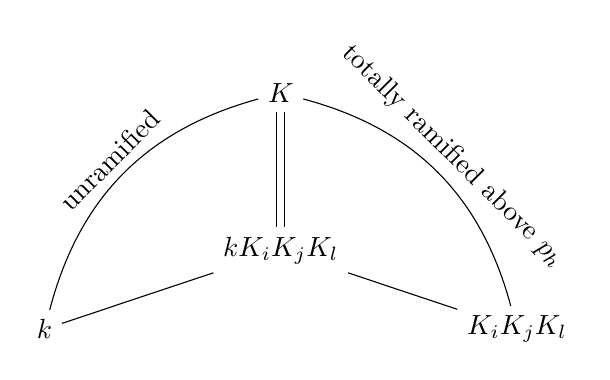
\begin{tikzpicture}
  \node (a) at (0,4)  {$K$};
  \node (b) at (0,2)  {$kK_iK_jK_l$};
  \node (c) at (-3,1)  {$k$};
  \node (d) at (3,1)  {$K_iK_jK_l$};
  \draw[transform canvas={xshift=-1.5pt}] (a) -- (b);
  \draw[transform canvas={xshift=1.5pt}] (b) -- (a);
  \draw   (b) --  (c)
   (b) -- (d);
  \draw[bend left](c) to node [above , sloped]{\text{unramified}}(a);
  \draw[bend right](d) to node [above , sloped]{\text{totally ramified above $p_h$}}(a);
\end{tikzpicture}
\end{center}
%Přidat zvláštní lemma o Galoisových grupách K_iK_jK_l/K_i a podobně kvůli čitelnosti?

\begin{prop}\label{degrees}
We have $a_i=[k\cap K_i:\Q]$, $r_i=[K:kK_i]$, $|T_i|=a_i\frac{m}{r_i}$,  $s_{ij}=[K:kK_iK_j]$. Also $[K_i:k\cap K_i]=\frac{m}{r_i}$, $[K_iK_j:k\cap K_iK_j]=\frac{m}{s_{ij}}$ and $[K_iK_jK_l:k\cap K_iK_jK_l]=m$.
\end{prop}
\begin{proof}
Since
\begin{equation*}
\begin{split}
\Gal(K/K_i)&=\Gal(K/K_iK_jK_l\cap K_iK_jK_h\cap K_iK_lK_h)\\
&=\Gal(K/K_iK_jK_l)\cdot \Gal(K/K_iK_jK_h)\cdot \Gal(K/K_iK_lK_h)
= T_jT_lT_h
\end{split}
\end{equation*} 
%$$\Gal(K/K_i)\cong \Gal(K/\Q)/\Gal(K_i/\Q)\cong T_1T_2T_3T_4/T_i\cong T_jT_lT_h$$
 and $\Gal(K/k)=H$, it follows that $\Gal(K/k\cap K_i)= T_jT_lT_h\cdot H$. Now consider the short exact sequence %(clearly $\ker \pi_i=T_jT_lT_h$) 
$$0\to H\cap \ker \pi_i\to H \xrightarrow{\restr{\pi_i}{H}} \pi_i(H)\to 0.$$
It follows that $|\pi_i(H)|=\frac{m}{r_i}$ and $$\pi_i(H)\cong \frac{H}{H\cap \ker \pi_i}=\frac{H}{H\cap T_jT_lT_h}\cong \frac{T_jT_lT_h\cdot H}{T_jT_lT_h}= \frac{\Gal(K/k\cap K_i)}{\Gal(K/K_i)}\cong \Gal(K_i/k\cap K_i).$$
Therefore 
$$[k\cap K_i:\Q]=\frac{|\Gal(K_i/\Q)|}{|\Gal(K_i/k\cap K_i)|}=\frac{|T_i|}{|\pi_i(H)|}=a_i$$
%$$[k\cap K_i:\Q]=\frac{|T_1T_2T_3T_4|}{|T_jT_lT_h\cdot H|}=\frac{|T_1T_2T_3T_4|\cdot |H\cap T_jT_lT_h|}{|T_jT_lT_h|\cdot |H|}=\frac{|T_i|}{|\pi_i(H)|}=a_i.$$
and
$$[K:kK_i]=\frac{|\Gal(K/k)|}{|\Gal(kK_i/k)|}=\frac{|H|}{|\Gal(K_i/k\cap K_i)|}=\frac{m}{|\pi_i(H)|}=r_i.$$
Putting everything together, we obtain $$|T_i|=[K_i:k\cap K_i]\cdot[k\cap K_i:\Q]=a_i|\pi_i(H)|=a_i\frac{m}{r_i}.$$
Next, we also have 
\begin{equation*}
\begin{split}
\Gal(K/K_iK_j)&=\Gal(K/K_iK_jK_l\cap K_iK_jK_h)\\
&=\Gal(K/K_iK_jK_l)\cdot \Gal(K/K_iK_jK_h)= T_lT_h
\end{split}
\end{equation*} 
%$$\Gal(K/K_iK_j)\cong \Gal(K/\Q)/\Gal(K_iK_j/\Q)\cong T_1T_2T_3T_4/T_iT_j\cong T_lT_h,$$
so that $\Gal(K/k\cap K_iK_j)=T_lT_h\cdot H$. Thus we can consider the short exact sequence 
$$0\to H\cap \ker \pi_i\pi_j\to H \xrightarrow{\restr{\pi_i\pi_j}{H}} \pi_i\pi_j(H)\to 0$$
to conclude that $|\pi_i\pi_j(H)|=\frac{m}{s_{ij}}$ and 
\begin{equation*}
\begin{split}
\pi_i\pi_j(H)&\cong \frac{H}{H\cap \ker \pi_i\pi_j}=\frac{H}{H\cap T_lT_h}\cong \frac{T_lT_h\cdot H}{T_lT_h}\\
&\cong \frac{\Gal(K/k\cap K_iK_j)}{\Gal(K/K_iK_j)}\cong \Gal(K_iK_j/k\cap K_iK_j).
\end{split}
\end{equation*}
Then it follows that 
$$[K:kK_iK_j]=\frac{|\Gal(K/k)|}{|\Gal(kK_iK_j/k)|}=\frac{|H|}{|\Gal(K_iK_j/k\cap K_iK_j)|}=\frac{m}{\pi_i\pi_j(H)}=s_{ij}.$$
The last part of the statement is a consequence of Lemma \ref{comp}, since we have $$\Gal(K_iK_jK_l/k\cap K_iK_jK_l)\cong \Gal(kK_iK_jK_l/k)=\Gal(K/k)=H.$$
Finally note that in the same way as above, we could show that $$\pi_i\pi_j\pi_l(H)\cong \frac{H}{H\cap T_h}\cong H$$
(since Lemma \ref{comp} implies that $|H\cap T_h|=1$).
%Finally note that in the same way as above, we could show that $$\pi_i\pi_j\pi_l(H)\cong \Gal(K_iK_jK_l/k\cap K_iK_jK_l).$$
\end{proof}
\begin{center}
\begin{tikzpicture}
  \node (a) at (0,4)  {$K$};
  \node (b) at (0,2)  {$kK_i$};
  \node (c) at (-2,0)  {$k$};
  \node (d) at (2,0)  {$K_i$};
  \node (e) at (0,-2)  {$k\cap K_i$};
  \node (f) at (0,-4)  {$\Q$};
  \draw   (a) -- node [left]{$r_i$} (b) -- node [above left]{$\frac{m}{r_i}$} (c) -- (e) -- node [below right]{$|\pi_i(H)|$} (d) -- node [above right]{$\frac{|T_j\times T_l\times T_h|}{r_i}$} (b)
  (e) -- node [left]{$a_i$} (f);
\end{tikzpicture}
\qquad
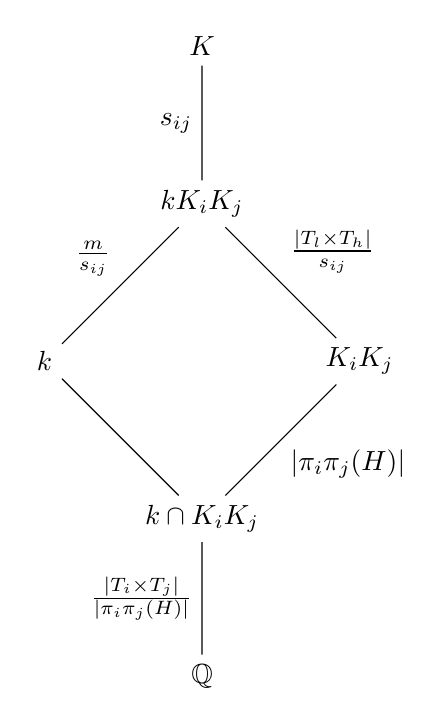
\begin{tikzpicture}
  \node (a) at (0,4)  {$K$};
  \node (b) at (0,2)  {$kK_iK_j$};
  \node (c) at (-2,0)  {$k$};
  \node (d) at (2,0)  {$K_iK_j$};
  \node (e) at (0,-2)  {$k\cap K_iK_j$};
  \node (f) at (0,-4)  {$\Q$};
  \draw   (a) -- node [left]{$s_{ij}$} (b) -- node [above left]{$\frac{m}{s_{ij}}$} (c) -- (e) -- node [below right]{$|\pi_i\pi_j(H)|$} (d) -- node [above right]{$\frac{|T_l\times T_h|}{s_{ij}}$} (b)
  (e) -- node [left]{$\frac{|T_i\times T_j|}{|\pi_i\pi_j(H)|}$} (f);
\end{tikzpicture}
%\vspace{3\baselineskip}
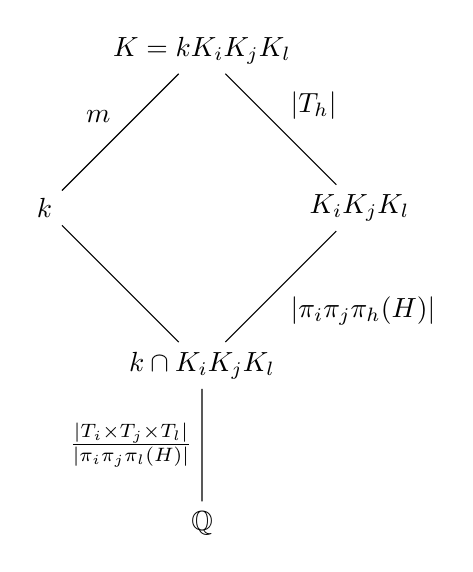
\begin{tikzpicture}
  \node (a) at (0,2)  {$K=kK_iK_jK_l$};
  \node (c) at (-2,0)  {$k$};
  \node (d) at (2,0)  {$K_iK_jK_l$};
  \node (e) at (0,-2)  {$k\cap K_iK_jK_l$};
  \node (f) at (0,-4)  {$\Q$};
  \draw   (a) -- node [above left]{$m$} (c) -- (e) -- node [below right ]{$|\pi_i\pi_j\pi_h(H)|$} (d) -- node [above right]{$|T_h|$} (a)
  (e) -- node [left]{$\frac{|T_i\times T_j\times T_l|}{|\pi_i\pi_j\pi_l(H)|}$} (f);
\end{tikzpicture}
\end{center}

\begin{cor}\label{compcap}
We have $[k\cap K_iK_j:\Q]=a_ia_j\frac{m}{r_ir_j}s_{ij}$, $[k\cap K_iK_jK_l:\Q]=a_ia_ja_l\frac{m^2}{r_ir_jr_l}$ and $[k:\Q]=a_1a_2a_3a_4\frac{m^3}{r_1r_2r_3r_4}$.
\end{cor}
\begin{proof}
This follows from the computations
$$[k\cap K_iK_j:\Q]=\frac{[K_iK_j:\Q]}{[K_iK_j:k\cap K_iK_j]}=\frac{|T_i|\cdot|T_j|}{m/s_{ij}}=a_ia_j\frac{m}{r_ir_j}s_{ij},$$
$$[k\cap K_iK_jK_l:\Q]=\frac{[K_iK_jK_l:\Q]}{[K_iK_jK_l:k\cap K_iK_jK_l]}=\frac{|T_i|\cdot|T_j|\cdot|T_l|}{m}=a_ia_ja_l\frac{m^2}{r_ir_jr_l}$$
and
\begin{equation*}
\begin{split}
[k:\Q]&=[k\cap K_i:\Q]\cdot [k:k\cap K_i]=a_i\cdot [kK_i:K_i]=a_i\frac{[K:K_i]}{[K:kK_i]}\\
&=a_i\frac{|T_j|\cdot|T_l|\cdot|T_h|}{r_i}=
a_1a_2a_3a_4\frac{m^3}{r_1r_2r_3r_4}.
\end{split}
\end{equation*}

\end{proof}
\begin{lemma}\label{coprime}
We have $$s_{ij}=\gcd(r_i,r_j),$$ $$\gcd(r_i,r_j,r_l)=1$$ (this is also equivalent to $\lcm\left(\frac{m}{r_i},\frac{m}{r_j},\frac{m}{r_l}\right)=m$ and to $\gcd(s_{ij},r_l)=1$) and $$s_{ij}\frac{m}{r_ir_j}=\gcd(\frac{m}{r_i},\frac{m}{r_j}).$$
\end{lemma}
\begin{proof}
It follows from Proposition \ref{degrees} that $s_{ij}\mid r_i, s_{ij}\mid r_j$ and from its proof that $|\pi_i(H)|=\frac{m}{r_i}$, $|\pi_i\pi_j(H)|=\frac{m}{s_{ij}}$ and $|\pi_i\pi_j\pi_l(H)|=m$. The cyclicity of $H$ then implies
$$\frac{m}{s_{ij}}=|\pi_i\pi_j(H)|=|\langle\pi_i\pi_j(\tau)\rangle|=|\langle\pi_i(\tau)\pi_j(\tau)\rangle|=\lcm\left(\frac{m}{r_i},\frac{m}{r_j}\right),$$
because $\langle\pi_i(\tau)\rangle=\pi_i(H)$ and any power of the product $\pi_i(\tau)\pi_j(\tau)$ is trivial if and only if the same power of both its factors is (since $G$ is the direct product of the $T_i$'s). 
%the elements $\pi_i(H),\pi_j(H)$ have different non-zero coordinates in $G$.
Now for any common divisor $t$ of $r_i,r_j$, we have $\frac{m}{s_{ij}}= \lcm\left(\frac{m}{r_i},\frac{m}{r_j}\right) \mid \frac{m}{t}$, which implies $t\mid s_{ij}$ and we are done.

Similarly, we have
$$m=|\pi_i\pi_j\pi_l(H)|=|\langle\pi_i\pi_j\pi_l(\tau)\rangle|=|\langle\pi_i(\tau)\pi_j(\tau)\pi_l(\tau)\rangle|=\lcm\left(\frac{m}{r_i},\frac{m}{r_j},\frac{m}{r_l}\right),$$
so if $t$ is any common divisor of $r_i,r_j,r_l$, we have $m=\lcm\left(\frac{m}{r_i},\frac{m}{r_j},\frac{m}{r_l}\right)\mid \frac{m}{t}$, which implies $t=1$.

Finally, using the first result, we have $s_{ij}\frac{m}{r_ir_j}=\frac{m}{\lcm(r_i,r_j)}$, which clearly divides both $\frac{m}{r_i}$ and $\frac{m}{r_j}$. Moreover, if $t$ is any common divisor of $\frac{m}{r_i}$ and $\frac{m}{r_j}$, then both $r_it$ and $r_jt$ divide $m$, hence $t\cdot\lcm(r_i,r_j)=\lcm(r_it,r_jt)\mid m$. Thus $t\mid \frac{m}{\lcm(r_i,r_j)}$ and we are done.
\end{proof}

\begin{prop}\label{gal}
We have 
\begin{equation*}
\begin{split}
\Gal(k/\Qbb)\cong
 \{\restr{\left(\sigma_1^{x_1}\sigma_2^{x_2}\sigma_3^{x_3}\sigma_4^{x_4}\right)}{k};~ & 0\leq x_1<a_1\frac{m}{r_1}, 0\leq x_2<a_2\frac{m}{r_2s_{34}}, \\ & 0\leq x_3<a_3\frac{m}{r_3r_4}s_{34},0\leq x_4<a_4\},
\end{split}
\end{equation*}
where each automorphism of $k$ determines the quadruple $(x_1,x_2,x_3,x_4)$ uniquely.
\end{prop}
\begin{proof}
By Corollary \ref{compcap}, the set on the right hand side has at most $|\Gal(k/\Qbb)|$ elements. Now let $\rho$ be any automorphism of $k$. If we can show that $\rho$ determines the quadruple $(x_1,x_2,x_3,x_4)$ belonging to the set on the right hand side uniquely, it will follow that the cardinalities agree and we will be done. Since $\Gal(k\cap K_4/\Q)$ is a cyclic group of order $a_4$ (by lemma \ref{degrees}) generated by $\restr{\sigma_4}{k\cap K_4}$ (as a quotient of $\Gal(K_4/\Q)=\langle \restr{\sigma_4}{K_4}\rangle$), there must exist a unique $x_4\in \Z$, $0\leq x_4<a_4$ such that $\rho$ and $\sigma_4^{x_4}$ have the same restrictions to $k\cap K_4$. Therefore $\rho\restr{\sigma_4^{-x_4}}{k}\in \Gal(k/k\cap K_4)$. 

Next, $\Gal(k\cap K_3K_4/k\cap K_4)$ is a cyclic group of order $\frac{[k\cap K_3K_4:\Q]}{[k\cap K_4:\Q]}=a_3\frac{m}{r_3r_4}s_{34}$ (by Corollary \ref{compcap}) generated by $\restr{\sigma_3}{k\cap K_3K_4}$ (as a quotient of $\Gal(K_3K_4/K_4)=\langle \restr{\sigma_3}{K_3K_4}\rangle$), so there must exist a unique $x_3\in \Z$, $0\leq x_3<a_3\frac{m}{r_3r_4}s_{34}$ such that $\rho\sigma_4^{-x_4}$ and $\sigma_3^{x_3}$ have the same restriction to $k\cap K_3K_4$. Therefore $\restr{\rho\sigma_3^{-x_3}\sigma_4^{-x_4}}{k}\in \Gal(k/k\cap K_3K_4)$.

Following the pattern, $\Gal(k\cap K_2K_3K_4/k\cap K_3K_4)$ is a cyclic group of order 
$$\frac{[k\cap K_2K_3K_4:\Q]}{[k\cap K_3K_4:\Q]}=a_2\frac{m}{r_2s_{34}}$$ (by Corollary \ref{compcap}) generated by $\restr{\sigma_2}{k\cap K_2K_3K_4}$ (as a quotient of $$\Gal(K_2K_3K_4/K_3K_4)=\langle \restr{\sigma_2}{K_2K_3K_4}\rangle),$$ so there must exist a unique $x_2\in \Z$, $0\leq x_2<a_2\frac{m}{r_2s_{34}}$ such that $\rho\sigma_3^{-x_3}\sigma_4^{-x_4}$ and $\sigma_2^{x_2}$ have the same restriction to $k\cap K_2K_3K_4$. Therefore $\restr{\rho\sigma_2^{-x_2}\sigma_3^{-x_3}\sigma_4^{-x_4}}{k}\in \Gal(k/k\cap K_2K_3K_4)$.

Finally, we have $$\Gal(k/k\cap K_2K_3K_4)\cong \Gal(kK_2K_3K_4/K_2K_3K_4)=\Gal(K_1K_2K_3K_4/K_2K_3K_4)=\langle\sigma_1\rangle$$
(using Lemma \ref{comp}), where the isomorphism is given by restriction. Since the order of $\sigma_1$ is $a_1\frac{m}{r_1}$, it follows that there must exist a unique $x_1\in \Z$, $0\leq x_1<a_1\frac{m}{r_1}$ such that $\rho\sigma_2^{-x_2}\sigma_3^{-x_3}\sigma_4^{-x_4}$ and $\sigma_1^{x_1}$ have the same restriction to $k$. Thus $\rho=\sigma_1^{x_1}\sigma_2^{x_2}\sigma_3^{x_3}\sigma_4^{x_4}$ and the proof is finished.
\begin{center}
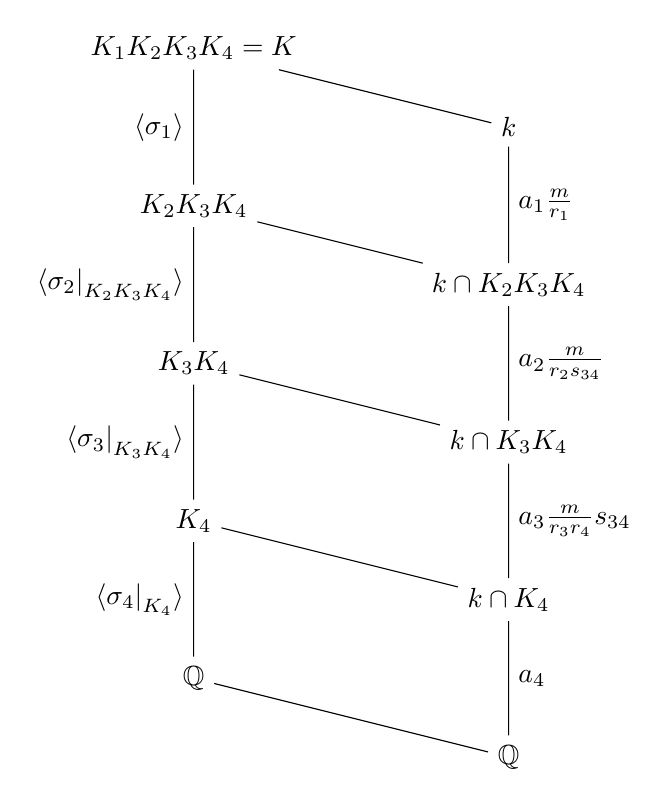
\begin{tikzpicture}
  \node (a) at (0,4)  {$K_1K_2K_3K_4=K$};
  \node (b) at (4,3)  {$k$};
  \node (c) at (0,2)  {$K_2K_3K_4$};
  \node (d) at (4,1)  {$k\cap K_2K_3K_4$};
  \node (e) at (0,0)  {$K_3K_4$};
  \node (f) at (4,-1)  {$k\cap K_3K_4$};
  \node (g) at (0,-2) {$K_4$};
  \node (h) at (4,-3)  {$k\cap K_4$};
  \node (i) at (0,-4) {$\Q$};
  \node (j) at (4,-5)  {$\Q$};
  \draw  (a) -- node [midway,left]{$\langle \sigma_1\rangle$} (c) -- node [midway,left]{$\langle \restr{\sigma_2}{K_2K_3K_4}\rangle$} (e) -- node [midway,left]{$\langle \restr{\sigma_3}{K_3K_4}\rangle$} (g) -- node [midway,left]{$\langle \restr{\sigma_4}{K_4}\rangle$} (i) -- (j) -- node [midway,right]{$a_4$} (h) -- node [midway,right]{$a_3\frac{m}{r_3r_4}s_{34}$} (f) -- node [midway,right]{$a_2\frac{m}{r_2s_{34}}$} (d) -- node [midway,right]{$a_1\frac{m}{r_1}$} (b) -- (a) 
  (c) -- (d)
  (e) -- (f)
  (g) -- (h);
\end{tikzpicture}
\end{center}
\end{proof}

\begin{lemma}
Without loss of generality, we can assume $\tau=\sigma_1^{a_1}\sigma_2^{a_2}\sigma_3^{a_3}\sigma_4^{a_4}$.
\end{lemma}
\begin{proof}
We know that $a_i=[T_i:\pi_i(H)]$, hence
$\pi_i(\tau)$ generates a subgroup of $T_i$ of index $a_i$. The cyclicity of $T_i$ then implies that $\pi_i(\tau)$ must be the $a_i$-th power of some generater of $T_i$, WLOG $\sigma_i$. The statement now follows, because $\tau$ is determined by its four projections.
\end{proof}

\section{The group of circular numbers}

Recall that $D^+$, the subgroup of totally positive elements of the group $D$ of circular numbers of a real abelian field $k'$ (using Lettl's modification of Sinnott's definition), has one generator $\eta_I$ for each nonempty subset $I\subseteq P$, where $P$ is the set of ramified primes of $k'$. (Since $k'$ is real, $D^+$ is also canonically isomorphic to the non-torsion part of $D$.) 

More explicitly, if we let $K'_i$ be the largest subfield of $K'$ (the genus field of $k'$ in the narrow sense) in which $p_i$ is the only ramified prime for any $i\in I$, we have
$$\eta_I=\text{N}_{\Qbb(\zeta_{\text{cond} \left(\prod_{i\in I}K'_i\right)})/\left(\prod_{i\in I}K'_i)\right)\cap k'}\left(1-\zeta_{\text{cond} \left(\prod_{i\in I}K'_i\right)}\right).$$
It is well known that $D^+$ is a $\Zbb[G]$-module of $\Zbb$-rank $[k:\Qbb]+|P|-1$. 

(In our case, we have $k'=k, K'=K, K'_i=K_i, |P|=4$, $\eta:=\eta_{\{1,2,3,4\}}$.)

%The generators of $D^+$ are subject to norm relations (which can be obtained by computing the norm of the generators to a subfield with less ramified primes) and for $|P|\geq 3$, also to the so-called Ennola relations, which are highly nontrivial relations that are not consequences of the norm relations.

%Our goal will be to find a basis of $D^+$ (it can then be easily modified in order to obtain a basis of the group of circular units). Such a basis is known only in a few very special cases though. We would like to construct it for general abelian fields as well, based only on the number of ramified primes.
\paragraph*{}
Our goal will be to find a basis of $D^+$ (it can then be easily modified in order to obtain a basis of the group of circular units). The generators of $D^+$ are subject to norm relations that correspond to the sum of all elements of the respective inertia groups $T_i$. Namely, let $$R_i=\sum_{u=0}^{a_i-1}\sigma_i^u,\, N_i=\sum_{u=0}^{\frac{m}{r_i}-1}\sigma_i^{ua_i}.$$ 
Then the norm operators from $k$ to a maximal subfield ramified at three primes can be given as $R_iN_i$ (i.e. the sum of all elements of $T_i$). If we denote the congruence corresponding to the canonical projection $\Z[G]\to \Z[G/H]$ by $\equiv$, then we have $N_4\equiv \sum_{u=0}^{m-1}\sigma_1^{ua_1}\sigma_2^{ua_2}\sigma_3^{ua_3}$.

Moreover, we will denote the congruence corresponding to the composition of canonical projections $\Z[G]\to \Z[G/H]\to \Z[G/H]/(R_1N_1,R_2N_2,R_3N_3,R_4N_4)$ by $\sim$, where $(R_1N_1,R_2N_2,R_3N_3,R_4N_4)$ is the ideal generated in $\Z[G/H]$ by the images of the elements $R_iN_i$. When we apply any element of this ideal to the highest generator $\eta$, we will obtain a multiplicative $\Z$-linear combination of circular units belonging to subfields with less ramified primes. We will make use of this extensively.

To construct a basis of $D^+$, we can take the union of all bases for the fields $$k\cap K_1K_2K_3,k\cap K_1K_2K_4,k\cap K_1K_3K_4,k\cap K_2K_3K_4$$ (which have three ramified primes, so we can use the results in [1]) and add in
\begin{equation*}
\begin{split}
c:&=[k:\Q]+3-\sum_{i,j,l}([k\cap K_iK_jK_l:\Q]+2)+\sum_{i,j}([k\cap K_iK_j:\Q]+1)-\sum_{i}[k\cap K_i:\Q]\\&=a_1a_2a_3a_4\frac{m^3}{r_1r_2r_3r_4}-\sum_{i,j,l}a_ia_ja_l\frac{m^2}{r_ir_jr_l}+\sum_{i,j}
a_ia_js_{ij}\frac{m}{r_ir_j}-\sum_{i}a_i+1
\end{split}
\end{equation*}
(by the principle of inclusion and exclusion due to the fact that these bases were constructed "inductively") conjugates of $\eta$. Then we will need to show how to obtain the missing conjugates of $\eta$ using the relations $$R_1N_1\sim 0, R_2N_2\sim 0, R_3N_3\sim 0, R_4\sum_{u=0}^{m-1}\sigma_1^{ua_1}\sigma_2^{ua_2}\sigma_3^{ua_3}\sim 0.$$

We will always refer to the conjugates of $\eta$ by their coordinates $x_1,x_2,x_3,x_4$ according to Proposition \ref{gal}. This allows for geometric interpretation.

\section{The case $r_1=r_2=a_3=r_4=1$}
(Note that in this case we have $s_{34}=1$.) %, therefore $$c=a_1a_2a_4\frac{m^3}{r_3}-\sum_{i,j,l}a_ia_ja_l\frac{m^2}{r_ir_jr_l}+\sum_{i,j}+a_ia_js_{ij}\frac{m}{r_ir_j}-\sum_{i}a_i+1.$$
\paragraph*{}
We will add all the conjugates of $\eta$ to our basis except the following cases:
\begin{itemize}
\item $x_1=a_1m-1$ or $x_2=a_2m-1$ or $x_3=\frac{m}{r_3}-1$,
\item $a_1\leq x_1 < a_1m-1, a_2(m-1)-1 \leq x_2 < a_2m-1, 0\leq x_3 < \frac{m}{r_3}-1, x_4=0$,
\item $0\leq x_1 < a_1, a_2(m-1) \leq x_2 < a_2m-1, 0\leq x_3 < \frac{m}{r_3}-1, x_4=0$.
\end{itemize}
These cases are all disjoint, so it's easy to see that the number of conjugaters of $\eta$ that we chose is exactly
$$((a_1m-1)a_2(m-2)+(a_1m-1)(a_2-1)+a_1+(a_4-1)(a_1m-1)(a_2m-1))\left(\frac{m}{r_3}-1\right)=c.$$
\paragraph*{}
First we will recover the cases $0<x_4<a_4$, $x_1=a_1m-1$ or $x_2=a_2m-1$ or $x_3=\frac{m}{r_3}-1$ using the relations $R_1N_1\sim 0, R_2N_2\sim 0, R_3N_3\sim 0$. From now on, we only need to deal with the cases where $x_4=0$.
\paragraph*{}
Next, we will recover the cases $$x_1=a_1m-1, 0\leq x_2 < a_2(m-1)-1, 0\leq x_3 <\frac{m}{r_3}-1$$ using the relation $R_1N_1\sim 0$ and subsequently the cases $$0\leq x_1 < a_1m-1, 0\leq x_2 < a_2(m-1)-1, 0\leq x_3 <\frac{m}{r_3}-1$$ and $$0\leq x_1 < a_1-1, x_2 = a_2(m-1)-1, 0\leq x_3 <\frac{m}{r_3}-1$$ using the relation $R_3N_3\sim 0$.
\paragraph*{}
Next, we will sequentially recover all the cases $$0\leq x_1 < a_1m-1, a_2(m-1)\leq x_2 < a_2m-1, 0\leq x_3 <\frac{m}{r_3}-1$$
using the relation $R_4\sum_{u=0}^{m-1}\sigma_1^{a_1u}\sigma_2^{a_2u}\sigma_3^u$. We can do this since any two conjugates of $\eta$ used in this relation differ by at least $a_2$ in their second coordinate. After this, we can recover the cases $$0\leq x_1 < a_1, x_2 = a_2m-1, 0\leq x_3 <\frac{m}{r_3}-1$$ using the relation $R_2N_2\sim 0$.
\paragraph*{}
Finally, we can use the relation $R_4\sum_{u=0}^{m-1}\sigma_1^{a_1u}\sigma_2^{a_2u}\sigma_3^u$ to recover the cases $$a_1 \leq x_1 <2a_1, x_2 =a_2m-1, 0\leq x_3 <\frac{m}{r_3}-1$$ and subsequently $R_4\sum_{u=0}^{m-1}\sigma_1^{a_1u}\sigma_2^{a_2u}\sigma_3^u$ to recover the cases $$a_1 \leq x_1 <2a_1, x_2 =a_2(m-1)-1, 0\leq x_3 <\frac{m}{r_3}-1.$$ By repeating these two steps $(m-2)$ more times, increasing the first coordinate by $a_1$ each time, we will recover all the conjugates.

\section{The case $a_1=a_2=r_3=r_4=1$}
(Recall that $n_i=\frac{m}{r_i}$.)

In this case, using Lemma \ref{coprime}, we have
\begin{equation*}
\begin{split}
c&=a_3\left(n_1-1\right)\left(n_2-1\right)\left(m-1\right)-\left(n_1-1\right)\left(n_2-1\right)+\gcd\left(n_1,n_2\right)-1\\
&+(a_4-1)\left(a_3\left(n_1-1\right)\left(n_2-1\right)m-\left(n_1-1\right)\left(n_2-1\right)\right).
\end{split}
\end{equation*}
We will add the following $c$ conjugates of $\eta$ to our basis:
\begin{itemize}
\item $0\leq x_1<n_1-1, 0\leq x_2<n_2-1, 0\leq x_3<a_3m-1, 0<x_4\leq a_4-1$,
\item $0\leq x_1<n_1-1, 0\leq x_2<n_2-1, 0\leq x_3<a_3(m-1)-1, x_4=0$,
\item $n_1-(\gcd\left(n_1,n_2\right)-1)\leq x_1\leq n_1-1, x_2=n_2-1, x_3=a_3m-1, x_4=0$.
\end{itemize}

\paragraph*{}
First we will recover the cases $0<x_4<a_4$, $x_1=n_1-1$ or $x_2=n_2-1$ or $x_3=a_3m-1$ using the relations $N_1\sim 0, N_2\sim 0, R_3N_3\sim 0$. From now on, we only need to deal with the cases where $x_4=0$.
\paragraph*{}
Next, we will recover the cases $0\leq x_3<a_3(m-1)-1$, $x_1=n_1-1$ or $x_2=n_2-1$ using the relations $N_1\sim 0, N_2\sim 0$. Now we can also use the relation $R_4\sum_{u=0}^{m-1}\sigma_1^{u}\sigma_2^{u}\sigma_3^{a_3u}\sim 0$ multiple times to recover the cases $$0\leq x_1\leq n_1-1, 0\leq x_2\leq n_2-1, a_3(m-1)\leq x_3<a_3m-1.$$
\paragraph*{}
At this moment, we are only missing all the cases with $x_3=a_3(m-1)-1$ and some of those with $x_3=a_3m-1$. 
Let's focus on the second kind. The conjugates with $x_3=a_3m-1$ (and $x_4=0$) can be visualized as a discrete rectangle with sides $n_1$ and $n_2$. It is easy to see that such a rectangle can be partitioned into $\gcd(n_1,n_2)$ diagonals, each containing $\lcm(n_1,n_2)$ elements (two conjugates lie in the same diagonal iff their quotient is a power of $\eta^{\sigma_1^v\sigma_2^v}$ for some $v\in\Z$). Now consider the relations $$T:=-\left(\sigma_3^{a_3-1}R_4\sum_{u=0}^{m-1}\sigma_1^{u}\sigma_2^{u}\sigma_3^{a_3u}\right)-\sigma_1^{\frac{m}{r_1}-2}\sigma_2^{\frac{m}{r_2}-2} R_3N_3$$
and
$$S_v:=\sum_{u=0}^{v}\sigma_1^{-u}\sigma_2^{-u}T \text{ for } v\in\Z.$$
Clearly $T\sim 0, S_v\sim 0$ for all $v\in\Z$. Also note that for any $v$, $\eta^{S_v}$ contains no conjugate with $x_3=a_3(m-1)-1$ and contains exactly one conjugate with $x_3=a_3m-1$ that we cannot recover yet minus $\sigma_3^{a_3m-1}$, and these two always lie on the same diagonal. Moreover, any conjugate sharing this diagonal can occur as the one with positive sign for suitable $v\in\Z$. Therefore, since we already have the conjugates $$n_1-(\gcd\left(n_1,n_2\right)-1)\leq x_1\leq n_1-1, \leq x_2=n_2-1, x_3=a_3m-1$$ in our basis, we can recover all the conjugates that share the same diagonal with any (and therefore all) of these.
\paragraph*{}
Now we can recover all the conjugates with $x_3=a_3m-1$ except $\lcm(n_1,n_2)$ of them, which share a diagonal. By using the relation $\sigma_1^{\gcd\left(n_1,n_2\right)-1}\left(S_v-S_w\right)\sim 0$ for suitable $v,w\in\Z$, it is clear that we can generate the difference of any two conjugates lying on this diagonal. Now let $$n_1':=\frac{n_1}{\gcd\left(n_1,n_2\right)}, \quad n_2':=\frac{n_2}{\gcd\left(n_1,n_2\right)}$$ and
note that in each column, there are exactly $n_1'$ conjugates lying on this diagonal, and in each row, there are exactly $n_2'$ conjugates lying on this diagonal. Moreover, we have $$\gcd\left(n_1',n_2'\right)=1$$ by construction,
so there exists an integer $z>0$ such that $$n_2'z\equiv 1\pmod{n_1'}.$$
Using the observation above, we can generate $n_2'z$ differences of conjugates lying on the last diagonal in such a way that we will obtain each of the conjugates in the row $x_1=0$ exactly $z$ times with a negative sign, each of the conjugates in the column $x_2=0$ exactly $\frac{n_2'z-1}{n_1'}$ times with a positive sign and finally one conjugate with a positive sign with $$x_1=n_1-(\gcd\left(n_1,n_2\right)-1)-1,x_2=n_2-1.$$
 %$\frac{\frac{m}{r_2}}{\gcd\left(\frac{m}{r_1},\frac{m}{r_2}\right)}$ conjugates with a negative sign evenly distributed among the row $x_1=0$,  $\frac{\frac{\frac{m}{r_2}}{\gcd\left(\frac{m}{r_1},\frac{m}{r_2}\right)}z-1}{\frac{\frac{m}{r_1}}{\gcd\left(\frac{m}{r_1},\frac{m}{r_2}\right)}}$ conjugates with a positive sign evenly distributed among the column $x_2=0$ and finally one conjugate with a positive sign with $$x_1=a_1\frac{m}{r_1}-(\gcd\left(\frac{m}{r_1},\frac{m}{r_2}\right)-1)-1,x_2=\frac{m}{r_2}-1.$$
We can keep this last one and get rid of the rest using the relations $N_1\sim 0$, $N_2\sim 0$. Using this last one, we can generate the rest of its diagonal in the same way as above. Hence we have recovered all the conjugates with $x_3=a_3m-1$. Finally, using the relation $R_3N_3\sim 0$, we can now recover all the conjugates with $x_3=a_3(m-1)-1$ and we are done.

%$$0\sim\left(\left(\sum_{u=0}^{m-1}\sigma_1^{ua_1}\sigma_2^{ua_2}\sigma_3^{ua_3}\right)+\sigma_1^{\frac{m}{r_1}-2}\sigma_2^{\frac{m}{r_2}-2}N_3\right)\left(\sum_{u=0}^{\frac{\frac{m}{r_1}-3}{2}}\sigma_1^{2u}\right)$$

\section{The case $a_1=a_2=a_3=r_4=1, s_{12}=s_{13}=s_{23}=1,\gcd(n_1,n_2,n_3)=1 (\iff m=r_1r_2r_3)$}
In this case, using Lemma \ref{coprime}, we have
%case when some n_i are coprime
\begin{equation*}
\begin{split}
c=&a_4n_1n_2n_3-\frac{n_1n_2n_3}{m}-a_4(n_1n_2+n_1n_3+n_2n_3)+a_4-2+a_4(n_1+n_2+n_3)+\\
&\gcd(n_1,n_2)+\gcd(n_1,n_3)+\gcd(n_2,n_3)\\
=&(a_4-1)(n_1-1)(n_2-1)(n_3-1)+(n_1-1)(n_2-1)(n_3-2)+\\
&(n_1n_2-(\gcd(n_1,n_3)+1)n_2-(n_1-\gcd(n_1,n_3)-1)+\gcd(n_2,n_3)+\gcd(n_1,n_2)-2.
\end{split}
\end{equation*}
We will add the following $c$ conjugates of $\eta$ to our basis:
\begin{itemize}
\item $0\leq x_1<n_1-1, 0\leq x_2<n_2-1, 0\leq x_3<a_3m-1, 0<x_4\leq a_4-1$,
\item $0\leq x_1<n_1-1, 0\leq x_2<n_2-1, 1\leq x_3<n_3-1, x_4=0$,
\item $0\leq x_1< n_1-\gcd(n_1,n_3)-1, 0\leq x_2<n_2-1, x_3=0, x_4=0$,
\item           $x_1=n_1-\gcd(n_1,n_3)-1, 0\leq x_2<\gcd(n_2,n_3)+\gcd(n_1,n_2)-2, x_3=0, x_4=0$.
\end{itemize}

First we will recover the cases $0<x_4<a_4$, $x_1=n_1-1$ or $x_2=n_2-1$ or $x_3=a_3m-1$ using the relations $N_1\sim 0, N_2\sim 0, N_3\sim 0$. From now on, we only need to deal with the cases where $x_4=0$. Next, we will recover the cases $1< x_3 \leq n_3-1$, $x_1=n_1-1$ or $x_2=n_2-1$ using the relations $N_1\sim 0, N_2\sim 0$ and the cases $x_3=0$, $0\leq x_1< n_1-\gcd(n_1,n_3)-1$, $x_2=n_2-1$ using the relation $N_2\sim 0$.
\paragraph*{}
At this moment, we are only missing all the cases with $x_3=1$ and some of those with $x_3=0$. From now on, we will only focus on recovering those with $x_3=0$ (without explicitly mentioning it anymore), because once we have those, we can recover those with $x_3=1$ using just the relation $N_3\sim 0$.
\paragraph*{}
Now let $t,u,v\in\Z$ be such that $n_1=tu,n_2=tv$ and $\gcd(u,v)=1$, i.e. $t=\gcd(n_1,n_2)$. Since $s_{12}=1$, this implies that $m=\lcm(n_1,n_2)=tuv$. But we also have the conditions $s_{13}=s_{23}=1$ which imply that $tuv=m=\lcm(tu,n_3)=\lcm(tv,n_3)$. Next, since $\gcd(n_1,n_2,n_3)=1$, $t$ must be coprime with $n_3$, therefore $n_3\mid uv$. Finally, the equalities $$\lcm(tu,n_3)=\frac{tun_3}{(tu,n_3)}=tuv=\frac{tvn_3}{(tv,n_3)}=\lcm(tv,n_3)$$
show that $u,v\mid n_3$, hence $uv=\gcd(u,v)\mid n_3$ and $n_3=uv$. It follows that $t=r_3,u=r_2,v=r_1$ (and thus $u=\gcd(n_1,n_3)$ and $v=\gcd(n_2,n_3)$. Thanks to the symmetry, we will assume $1<t<u<v$ (if any of $t,u,v$ would equal $1$, this case could be reduced to one of the previous two). We will also write $\uo:=u\pmod{t}$, $\vo:=v\pmod{t}$ (so that $\uo,\vo\in\{1,2,\dots,t-1\}$) and similarly for other expressions. In particular, the expressions $\uo/\vo$ and $\vo/\uo$ will be regarded modulo $t$ as well.
% It follows that also $\gcd(t,u)=\gcd(t,v)=1$ (and therefore $u=\gcd(n_1,n_3)$ and $v=\gcd(n_2,n_3)$. In fact, 
\paragraph*{}
The conjugates with $x_3=0$ (and $x_4=0$) can be visualized as a discrete rectangle with sides $n_1$ and $n_2$. Since for each $x_4$, there are $n_3$ rectangles in total, the relation $R_4\sum_{u=0}^{m-1}\sigma_1^{u}\sigma_2^{u}\sigma_3^{u}$ must contain $\frac{m}{n_3}=r_3$ conjugates in each of these rectangles. Thus the expression $\eta^{T'}$, where  $$T':=R_4\sum_{q=0}^{m-1}\sigma_1^{q}\sigma_2^{q}\sigma_3^{q}-\sum_{q=0}^{r_3-1} \sigma_1^{1+q n_3}\sigma_2^{1+q n_3}N_3 $$
(clearly $T'\sim 0$), contains only conjugates we have already recovered and those with $x_3=0$. More specifically, if we let $T$ be the sum of the automorphisms contained in  $R_4\sum_{u=0}^{m-1}\sigma_1^{u}\sigma_2^{u}\sigma_3^{u}$ with $x_3=0$, i.e. $T=\sum_{q=0}^{r_3-1}\sigma_1^{qn_3}\sigma_2^{qn_3}$, then $\eta^{(1-\sigma_1\sigma_2)T-T'}$ contains only conjugates which we have already recovered.
\paragraph*{}
Now we will decompose our rectangle (with $x_3=x_4=0$) into $t\times t$ rectangular blocks of height $u$ and width $v$ in the obvious way. In the following, by a big row (resp. big column) we will understand a row of blocks (resp. columns), that is $t$ consecutive blocks next to (resp. above) each other. Since $u,v\mid n_3$ and the conjugates contained in $\eta^T$ are given by $\sigma_1^{qn_3}\sigma_2^{qn_3}$ for $0\leq q \leq r_3-1$, the Chinese remainder theorem implies that $\eta^T$ contains exactly one conjugate in every big row (resp. big column), and these have the same relative position in each of the respective blocks (determined only by $n_3 \mod t$). We can be even more precise: the horizontal distance between $\eta^{\sigma_1^{qn_3}\sigma_2^{qn_3}}$ and $\eta^ {\sigma_1^{(q+1)n_3}\sigma_2^{(q+1)n_3}}$ for $0\leq q \leq r_3-1$ is exactly $\uo\cdot v$, i.e. $\uo$ blocks, and the vertical distance between them is exactly $\vo\cdot u$, i.e. $\vo$ blocks (again this follows easily from the Chinese remainder theorem). It follows that the horizontal distance between any two conjugates in $\eta^T$ with a vertical distance of one block is $\uo/\vo$ blocks.
\paragraph*{}
Let $Q$ be the quotient module of $D^+$ by the conjugates we can already recover (including those living in the maximal subfields ramified at three primes), regarded as $\Z$-modules (i.e. forgetting the $G$-structure, otherwise the quotient would be trivial). We will write $Q$ additively and for the remainder of this section, all equalities between (classes of) conjugates will be regarded as if in $Q$.
%From now on, we will regard the elements of our rectangle as their images in the quotient module of $\Z[G/H]/(N_1,N_2,N_3,N_4)$ by the $\Z$-module of the conjugates we can already recover (including those living in the maximal subfields ramified at three primes). We will call this quotient module $Q$.
\paragraph*{}
Showing that we have indeed chosen a basis now amounts to showing that the class of each conjugate in our rectangle is trivial in $Q$. For all $2\leq q\leq t+1$, we will denote the class of $\eta^{\sigma_1^{tu-2}\sigma_2^{q-2}}$ by $X_q$ and we will also put $X_{q'}:=X_q$ for all $q'\in\Z$, $q'\equiv q\pmod{t}$. Also for all $v+t-2\leq q\leq tv-1$ we will denote the class of $\eta^{\sigma_1^{(t-1)u-1}\sigma_2^q}$ by $Y_q$. We will refer to the set of these $\eta^{\sigma_1^{(t-1)u-1}\sigma_2^q}$ with $v+t-2\leq q\leq tv-1$ as the critical line. Now it suffices to show that $X_q=0$ for all $1\leq q\leq t$ and $Y_q=0$ for all $v+t-2\leq q\leq tv-1$.
\paragraph*{}
It is easy to see that our rectangle can be partitioned into $t=\gcd(n_1,n_2)$ (2D) diagonals, each going through exactly one of $\eta^{\sigma_1^{tu-2}\sigma_2^{q-2}}$ for $2\leq q\leq t+1$ (two conjugates lie in the same diagonal iff their difference is a power of $\eta^{\sigma_1^q\sigma_2^q}$ for some $q\in\Z$). We will use this together with the fact that $\eta^{(1-\sigma_1\sigma_2)T}$ is trivial in $Q$ to find the classes of all conjugates in our rectangle in terms of $X_q,Y_q$. More specifically, if $\eta^{\sigma_1^{x_1}\sigma_2^{x_2}(1-\sigma_1\sigma_2)T}$ contains no elements from the critical line, it is just a difference of two conjugates, hence their classes are the same. On the other hand, if it contains $Y_{q}$ for some $q$ and a difference of two conjugates, the classes of these two conjugates differ only by $\pm Y_{q}$ (depending on the sign of $Y_{q}$ in $\eta^{\sigma_1^q\sigma_2^r(1-\sigma_1\sigma_2)T}$). Using the earlier observations, we can see that these are the only options, hence it follows that by going along each of the $t$ 2D diagonals starting at $\eta^{\sigma_1^{tu-2}\sigma_2^{q-2}}$ for $2\leq q\leq t+1$, will will obtain that %the class of $\eta^{\sigma_1^q\sigma_2^r$
$$
[\eta^{\sigma_1^{x_1}\sigma_2^{x_2}}]=
\begin{cases}
0 \quad &\!\begin{aligned} \text{ if }  &x_1<t(u-1)-1\\ &\text{ or } x_1=t(u-1)-1, x_2< v+t-2 \end{aligned}\\
Y_{x_2} \quad &\text{ if } x_1=t(u-1)-1, v+t-2\leq x_2 \\
X_{-x_1+x_2+1} \quad &\!\begin{aligned}\text{ if } & t(u-1)-1\leq x_1<tu-1 \\&
 \text{ or }  x_1=tu-1, x_2\equiv q+\uo/\vo\cdot v\pmod{tv} \\
 &\text{ for some } 0\leq q<v+t-2  \end{aligned}\\
X_{-x_1+x_2+1}-Y_{x_2+(t-\uo/\vo)\cdot v} \quad &\!\begin{aligned}\text{ if } & x_1=tu-1, x_2\not\equiv q+\uo/\vo\cdot v\pmod{tv} \\
&\text{ for any } 0\leq q<v+t-2\end{aligned}\\
\end{cases}
$$
for any $0\leq x_1\leq tu-1, 0\leq x_2\leq tv-1$. Note that this implies that the action of $\sigma_1^{-x_1}\sigma_2^{x_2}$ on $X_q$ results in $X_{q+x_1+x_2}$ (unless the result is $0$ and ignoring all the $Y$'s.
%$X_q^{\sigma_2^{x_2}}=X_{q+x_2}$ for any $q,x_2$.

\paragraph*{}
Using the relation $N_1\sim 0$, we obtain the equation $u\cdot (X_1+\dots+X_t)=0$, and similarly the relation $N_2\sim 0$ implies $v\cdot (X_1+\dots+X_t)=0$, as well as $Y_{v+t-2}+\dots+Y_{tv-1}=0$. Since $\gcd(u,v)=1$, this implies $X_1+\dots+X_t=0$ be Bezout's identity. We will put $\beta=X_1+\dots+X_t$.
\paragraph*{}
%Next, note that for any set of conjugates, 
%Next, for $0\leq q \leq t-3$, we will put $$\Gamma_q:=\sum_{r=0}^{t-\uo/\vo-1}\sum_{p=1}^{\uo}X_{\overline{q+p-rv}}$$
%and $$\Delta:=\sum_{r=0}^{t-1}r\cdot\sum_{p=1}^{\uo}X_{\overline{p-rv}}.$$
Next, for $0\leq q \leq t-3$, we can see that taking the sum of all conjugates with $x_2=q+r\cdot \uo/\vo\cdot v$ for $0\leq r\leq t-\uo/\vo-1$ (using the relation $N_1\sim 0$) will result in $0$ in $Q$. By construction, all the $Y$'s involved will cancel out, and since $(t-\uo/\vo)\cdot v\equiv -\vo \pmod{t}$, this implies (using $\beta=0$) that $\Gamma_q=0$ in $Q$, where
$$\Gamma_q:=\sum_{r=0}^{t-\uo/\vo-1}\sum_{p=1}^{\uo}X_{\overline{q+p-rv}}.$$
Similarly, taking the sum of all conjugates with $r\cdot \uo/\vo\cdot v\leq x_2\leq v-1+r\cdot \uo/\vo\cdot v$ times $r$ for $0\leq r\leq t-\uo/\vo-1$ gives us $0$ (again using $N_1\sim 0$), hence so does summing over all such $r$ (where by construction all the $Y$'s involved cancel out except for one of each, and their sum is zero anyway). Therefore we have (by using $(t-\uo/\vo)\cdot v\equiv -\vo \pmod{t}$ and $\beta=0$ again) $\Delta=0$ in $Q$, where
$$\Delta:=\sum_{r=0}^{t-1}r\cdot\sum_{p=1}^{\uo}X_{\overline{p-rv}}.$$
%It's easy to check that all the $Y$'s cancel out in both of them.%, and that any shift in the indices in $\Gamma$ by $1,2,\dots,t-3$ will also result in a valid relation.
\paragraph*{}
Now we will construct a matrix $M$ of type $t\times t$ as follows:
\begin{itemize}
\item The first row will consist of all 1's (corresponding to the relation $\beta$).
%\item The second row will correspond to the relation $\Gamma$.
\item The $q$-th row for $2\leq q\leq t-1$ will correspond to the relation $\Gamma_{q-2}$.
\item The last row will correspond to the relation $\Delta$.
\end{itemize}

Since the rows of $M$ are the coefficients of valid equations in $Q$, we have $M\cdot X^T=0$, where $X=(X_1,\dots,X_t)$. We will show that $M$ is unimodular, i.e. invertible over $\Z$, from which it will follow that $X=0$. To do that, we will first need to describe $M$ in a better way.

\paragraph*{}
Let $L$ be the localization of the quotient ring $\Z[x]/(1+x+x^2+\dots+x^{t-1})$ at the multiplicative subset generated by $x-1$ and $x^{t-\uo}-1$. (By abuse of notation, we will denote the class of $x$ in $L$ also by $x$). Note that since $$\gcd(x^t-1,x^q-1)=x^{\gcd(t,q)}-1$$ for any $q\in\Z$ and $\gcd(t,1)=\gcd(t,t-\uo)=1$, we have $$\gcd(1+x+x^2+\dots+x^{t-1},x-1)=\gcd(1+x+x^2+\dots+x^{t-1},x^{t-\uo}-1)=1,$$ so that $x-1$ nor $x^{t-\uo}-1$ are zero-divisors, hence $L$ is nontrivial. Moreover let $$D(x):=\sum_{q=1}^{t-1}q\cdot x^q\in L.$$

\begin{lemma}
We have $D(x)\cdot(x-1)=t$.
\end{lemma}
\begin{proof}
This follows from the computation
\begin{equation*}
\begin{split}
D(x)\cdot(x-1)&=\sum_{q=1}^{t-1} q\cdot x^{q+1}-\sum_{q=1}^{t-1} q\cdot x^q=\sum_{q=2}^{t} (q-1)\cdot x^{q}-\sum_{q=1}^{t-1} q\cdot x^q\\
&=\sum_{q=1}^{t-1} (q-1)\cdot x^{q}-\sum_{q=1}^{t-1} q\cdot x^q-(t-1)x^t\\
&=-\sum_{q=1}^{t-1} x^{q}-x^t+t\cdot x^t\\
&=-\sum_{q=1}^{t} x^{q}+t\\
&=t.
\end{split}
\end{equation*}
\end{proof}

\begin{lemma}
The coefficients of $\Gamma_q$ are (up to a multiple of $\beta$) the coefficients of the polynomial $x^q\cdot P(x)$ and the coefficients of $\Delta$ are (up to a multiple of $\beta$) the coefficients of the polynomial $D\cdot P(x),$ where
$$P(x):=-x^{\uo}\cdot (1+x+x^2+\dots+x^{\vo-1})\in L$$
(where the coefficient at $X_{q+1}$ corresponds to the coefficient at $x^q$).
\end{lemma}
\begin{proof}
Since a cyclic shift of the indices of $X_q$ corresponds to multiplication by $x$ in $L$ and $x^m=1$ in $L$, the coefficients of $\Gamma_q$ (up to a multiple of $\beta$) are
\begin{equation*}\label{Gamma}
\begin{split}
&x^q\cdot(1+x+\dots+x^{\uo-1})(1+x^{m-\uo}+x^{2(m-\uo)}+\dots+x^{(t-\vo/\uo-1)(t-\uo)})\\
&=x^q\cdot\frac{x^{\uo}-1}{x-1}\cdot \frac{x^{(t-\vo/\uo)(t-\uo)}-1}{x^{t-\uo}-1}\\
&=x^q\cdot\frac{x^{\uo}-1}{x^{t-\uo}-1}\cdot \frac{x^{\vo}-1}{x-1}\\
&=-x^q\cdot x^{\uo}\cdot (1+x+x^2+\dots+x^{\vo-1})\\
&=P(x).
\end{split}
\end{equation*}
%Coming back to the coefficients in $\Gamma$, this means that % the second row of $M(t,u,v)$
%is exactly $$(1,\underbrace{0,\dots,0}_{\vo},\underbrace{1,\dots,1}_{t-\vo})$$ for $\uo=1$ and 
%incrementing $\uo$ by $1$ results in a cyclic shift of $\Gamma$ by $1$ to the right.
Similarly, using the substitution $y=x^{t-\uo}$ (so that $y^m=1$ in $L$), we can see that the coefficients of $\Delta$ (up to a multiple of $\beta$) are 
\begin{equation*}\label{Delta}
\begin{split}
&(1+x+\dots+x^{\uo-1})(1+x+\dots+x^{\vo-1})(x^{t-\uo}+2x^{2(t-\uo)}+\dots+(t-1)x^{(t-1)(t-\uo)})\\
&=\frac{x^{\uo}-1}{x-1}\cdot \frac{x^{\vo}-1}{x-1}\cdot y \cdot \frac{\partial}{\partial y} \left(\frac{y^{t}-1}{y-1}\right)\\
&=\frac{x^{\uo}-1}{x-1}\cdot \frac{x^{\vo}-1}{x-1}\cdot y \cdot \frac{ty^{t-1}(y-1)-(y^t-1)}{(y-1)^2}\\
&=\frac{x^{\uo}-1}{x-1}\cdot \frac{x^{\vo}-1}{x-1} \cdot \frac{t}{y-1}\\
&=\frac{t}{x-1}\cdot \frac{x^{\uo}-1}{x^{t-\uo}-1}\cdot \frac{x^{\vo}-1}{x-1}\\
&=D\cdot x^{\uo}\cdot\frac{x^{\vo}-1}{x-1}\\
&=D(x)\cdot P(x).
\end{split}
\end{equation*}
%Again, this means that incrementing $\uo$ by $1$ results in a cyclic shift of $\Delta$ by $1$ to the right.
\end{proof}

\begin{theorem}
$M$ is unimodular, hence $X=0$.
\end{theorem}
\begin{proof}
Let $\zt$ be a primitive $t$-th root of unity and let $C$ be the corresponding $t\times t$ character matrix, i.e. $C=(\zt^{r\cdot c})_{0\leq r,c<t}$. Then (after reindexing the dimensions of $M$ from $0$ to $t-1$) we have $M\cdot C=C'$, where $C_{0,0}=t$ and the $c-th$ column of $C'$ is
$$
\begin{pmatrix}
0\\ 
P(\zt^c) \\ 
\zt^c \cdot P(\zt^c) \\ 
\zt^{2c} \cdot P(\zt^c) \\ 
\vdots\\ 
\zt^{(t-3)c} \cdot P(\zt^c) \\ 
D(\zt^c) \cdot P(\zt^c)
\end{pmatrix}
$$
for $0<c<t$ (we don't need to specify the rest of the $0$-th column, since it doesn't influence the determinant of $C'$). Thus by taking out $P(\zt^c)$ from each of these columns, we get  (since multiplication by $\vo$ is an automorphism of $\Z/t$)
$$|\det C'|=|\det C''|\cdot\abs*{\prod_{0<c<t}P(\zt^c)}=|\det C''|\cdot\abs*{\prod_{0<c<t}-\zt^{c\uo}}\cdot\abs*{\prod_{0<c<t}\frac{\zt^{c\vo}-1}{\zt^c-1}}=|\det C''|,$$
where
$$C''=
\begin{pmatrix}
m& 0& \dots & 0 & \dots & 0\\ 
*& 1& \dots & 1 & \dots & 1\\ 
*& \zt& \dots & \zt^c & \dots & \zt^{t-1}\\ 
*& \zt^2& \dots & \zt^{2c} & \dots & \zt^{2(t-1)}\\ 
\vdots& \vdots&\ddots  & \vdots & \ddots & \vdots\\ 
*& \zt^{t-3}& \dots & \zt^{(t-3)c} & \dots & \zt^{(t-3)(t-1)}\\ 
*& D(\zt)& \dots & D(\zt^c) & \dots & D(\zt^{t-1})\\ 
\end{pmatrix}.
$$
On the other hand, if we take the matrix $C$, add all of its rows to the last one (thus creating $\begin{pmatrix}
t & 0 & 0& \dots &0
\end{pmatrix}$
there) and then add a suitable linear combination of rows $0,1,\dots, t-3$ to the $t-2$-th row times $-1$ using the equality
$$-\zt^{(t-2)c}+(t-1)\cdot\underbrace{\sum_{q=0}^{t-1}\zt^{qc}}_{=0}+\sum_{q=0}^{t-3}(q-t+1)\cdot\zt^{qc}=\sum_{q=0}^{t-1}q\cdot\zt^{qc},$$
so that the $t-2$-th row will become
$\begin{pmatrix}
*& D(\zt)& \dots & D(\zt^c) & \dots & D(\zt^{t-1}),
\end{pmatrix}$
we will obtain a matrix with the same determinant as $C''$. Since the elementary row operations preserve the determinant up to a sign, it follows that
$$|\det C|=|\det C''|=|\det C'|,$$ which together with the invertibility of $C$ (in fact it is well known that $\det C=\pm \sqrt{t^t}$) implies that $|\det M|=1$, as needed.
\end{proof}

\begin{cor}
We have $Y_q=0$ for all $v+t-2\leq q\leq tv-1$.
\end{cor}
\begin{proof}
%This now follows 
Take the sum of all conjugates with $x_2=r\cdot\uo/\vo\cdot v$ for $r=1$, then for $r=2$, and so on. In each sum all the conjugates are $0$ except the corresponding $Y_q$, so it must be zero as well. The result then follows by repeating the same procedure, only increasing $x_2$ in each of the sums by $1$ each time.
\end{proof}
\section{The module of relations}
\section{Construction of suitable abelian fields}
Let $m,a_1,a_2,a_3,a_4,r_1,r_2,r_3,r_4$ be positive integers such that 
$$m>1, r_i\mid m, \gcd(r_i,r_j,r_l)=1.$$
We will construct an infinite family of fields $k$ that satisfy all of our assumptions such that these integers correspond to the parameters in our problem of the same name.

First, we will fix distinct primes $p_1,p_2,p_3,p_4$ such that $p_i\equiv 1\pmod{ 2a_i\frac{m}{r_i}}$ (by Dirichlet's theorem on primes in arithmetic progressions, there are infinitely many ways of doing this). Then there exist even Dirichlet characters $\chi_i$ of conductors $p_i$ and orders $a_i\frac{m}{r_i}$ (namely, these can be given as $\chi_i:=\chi^{\frac{p_i-1}{a_im_i/r_i}}$, where $\chi$ is any generator of the cyclic group $\widehat{(\Z/p_i\Z)^\times}$ (note that $p_i>2$)).

Now let $K_i$ be the field associated to $\langle \chi_i\rangle$. Then $K_i$ is real (because $\chi_i$ is even) and $\Gal(K_i/\Q)$ is cyclic of order $a_i\frac{m}{r_i}$, say $\Gal(K_i/\Q)=\langle \sigma_i\rangle$. Moreover, since the conductors $p_i$ are coprime, the group $\langle \chi_1,\chi_2,\chi_3,\chi_4\rangle$ corresponds to the compositum field $K=K_1K_2K_3K_4$. By the theory of Dirichlet characters, $K$ is ramified exactly at primes $p_i$ (with inertia subgroups isomorphic to $\Gal(K_i/\Q)$) and $$\Gal(K/\Q)=\Gal(K_1/\Q)\Gal(K_2/\Q)\Gal(K_3/\Q)\Gal(K_4/\Q)=\langle\sigma_1,\sigma_2,\sigma_3,\sigma_4\rangle,$$
so that $[K:\Q]=a_1a_2a_3a_4\frac{m^4}{r_1r_2r_3r_4}$. Now let $\tau:=\sigma_1^{a_1}\sigma_2^{a_2}\sigma_3^{a_3}\sigma_4^{a_4}$ and let $k$ be the subfield of $K$ fixed by $\tau$. Since $k$ is a subfield of a compositum of real fields, it must also be real. In order to reach our goal, we now only need to prove the following theorem (it is not hard to see that we could have used the results from Lemma \ref{comp} and Proposition \ref{degrees} as definitions instead).

\begin{theorem}
In the above notation, we have $[K:k]=m$, $[K:kK_i]=r_i$, $[k\cap K_i:\Q]=a_i$ and $kK_iK_jK_l=K$ (i.e. $K$ is the genus field of $k$).
\end{theorem}
\begin{proof}
Using Lemma \ref{coprime} several times, we can compute
$$[K:k]=|\langle\tau\rangle|=\lcm\left(\frac{m}{r_i},\frac{m}{r_j},\frac{m}{r_l}\right)=m,$$
$$[K:kK_i]=|\langle\tau\rangle\cap \langle\sigma_j\sigma_l\sigma_h\rangle|=|\langle\tau^{a_im/r_i}\rangle|=r_i,$$
$$[k\cap K_i:/\Q]=[\langle\sigma_1,\sigma_2,\sigma_3,\sigma_4\rangle:\langle\tau,\sigma_j,\sigma_l,\sigma_h\rangle]=[\langle\sigma_1,\sigma_2,\sigma_3,\sigma_4\rangle:\langle\sigma_i^{a_i},\sigma_j,\sigma_l,\sigma_h\rangle]=a_i$$
and
$$[K:kK_iK_jK_l]=|\langle\tau\rangle\cap \langle\sigma_h\rangle|=|\langle\tau^{\lcm\left(\frac{m}{r_i},\frac{m}{r_j},\frac{m}{r_l}\right)}\rangle|=|\langle\tau^m\rangle|=1.$$
\end{proof}
\end{document}
